\documentclass[10pt]{article}
\usepackage[utf8]{inputenc}
\usepackage[spanish]{babel}
\usepackage{amsmath}
\usepackage{amsfonts}
\usepackage{amssymb}
\usepackage{graphics}
\usepackage{graphicx}
\usepackage[left=2cm,right=2cm,top=2cm,bottom=2cm]{geometry}
\usepackage{imakeidx}
\makeindex[columns=3, title=Alphabetical Index, intoc]
\usepackage{listings}
\usepackage{multicol}
\usepackage{changepage}
\usepackage{float}
\usepackage{cite}
\usepackage{url}
\usepackage{hyperref}
\usepackage{pdflscape}
\usepackage[document]{ragged2e}
\usepackage{xcolor,colortbl}

\hypersetup{
    colorlinks=true,
    linkcolor=blue,
    filecolor=magenta,
    urlcolor=blue,
}

\definecolor{Red}{rgb}{0.7,0,0}
\definecolor{LightCyan}{rgb}{0.88,1,1}
\definecolor{AquaCyan}{rgb}{0.2,1,0.5}
\definecolor{Gray}{gray}{0.85}
\definecolor{DarkBlue}{rgb}{0.1,0.1,0.5}

\definecolor{codegreen}{rgb}{0,0.6,0}
\definecolor{codegray}{rgb}{0.5,0.5,0.5}
\definecolor{codepurple}{rgb}{0.58,0,0.82}
\definecolor{backcolour}{rgb}{0.95,0.95,0.92}

\lstdefinestyle{mystyle}{
    backgroundcolor=\color{backcolour},
    commentstyle=\color{codegreen},
    keywordstyle=\color{magenta},
    numberstyle=\tiny\color{codegray},
    stringstyle=\color{codepurple},
    basicstyle=\ttfamily\footnotesize,
    breakatwhitespace=false,
    breaklines=true,
    captionpos=b,
    keepspaces=true,
    numbers=left,
    numbersep=5pt,
    showspaces=false,
    showstringspaces=false,
    showtabs=false,
    tabsize=3
}
\def\fillandplacepagenumber{%
 \par\pagestyle{empty}%
 \vbox to 0pt{\vss}\vfill
 \vbox to 0pt{\baselineskip0pt
   \hbox to\linewidth{\hss}%
   \baselineskip\footskip
   \hbox to\linewidth{%
     \hfil\thepage\hfil}\vss}}
\lstset{style=mystyle}

\title{Diferential Ecuation}

\author{A cargo del profesor: Luis Moctezuma Cervantes\\Escrito por: Adrian González Pardo}

\date{\today}

\newcommand\tab[1][1cm]{\hspace*{#1}}

\begin{document}
% Portada
%encabezado
\begin{minipage}{0.4\textwidth}
	\begin{flushleft}
		
\includegraphics[scale = 0.05]{logoescom.png}
	\end{flushleft}
\end{minipage}
\begin{minipage}{0.51\textwidth}
	\begin{flushright}
		
\includegraphics[scale = 0.055]{logoipn.png}
	\end{flushright}
\end{minipage}
\begin{center}
	\par\vspace{0.5cm}{
		\huge\textbf{Instituto Politécnico Nacional \\*[0.20cm] Escuela Superior de Cómputo}
	}
	\par\vspace{1cm}{
		\large\textbf{
		{Ecuaciones Diferenciales\\Profesor: Luis Moctezuma Cervantes\\Grupo: 1CM6\\Adrian González Pardo\\Semestre: 18/02}}
	}
	\par\vspace{1cm}{
		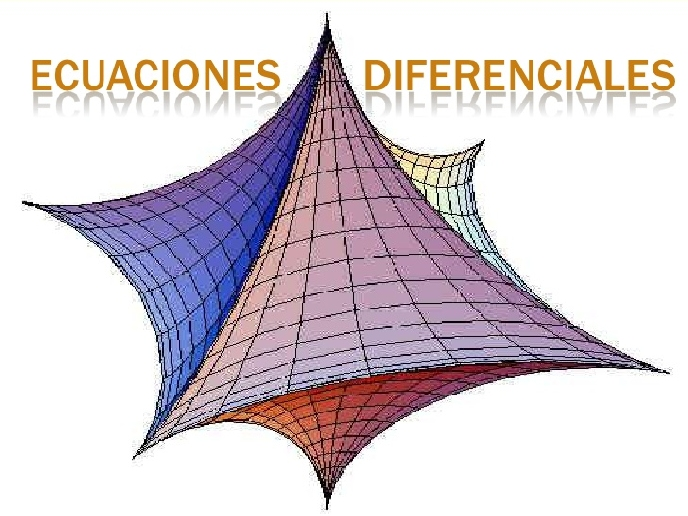
\includegraphics[scale=0.2]{ecuaciones.jpg}
	}
	\par\vspace{2cm}{
		Ultima fecha modificado: \today
	}
\end{center}

% Indice
\clearpage
\tableofcontents
\clearpage

%Contenido
\section{Introducción}
\subsection{Presentación}
Las ecuaciones diferenciales no son más que un conjunto de sistemas lineales o no lineales que representan modelo de comportamiento matemático, el cual puede ser aplicado en áreas como la ingeniería la cual puede servir para describir el comportamiento físico de un circuito electríco mediante las ecuaciones de voltaje de elementos lineales (resistencias, capacitadores e inductores), por otro lado igual puede ser aplicado en modelados matemáticos que puedan representar la medición estadística de una población de bacterias.\\
Ahora bien con el fin de facilitar el aprendizaje de estos temas se desarrollaran varias notas que se tomaron en el curso así como complemento de propía mano del escritor.
\subsection{Prerequisitos para la materia}
Si bien las matemáticas guardan una intima pero fuerte relación entre sus topicos es importante marcar algunos prerequisitos para poder dar seguimiento o poder tener un mejor entendimiento con la materia
\begin{center}
  \begin{tabular}{|p{5.5cm}|p{5.5cm}|}
    \hline
    Principios de Cálculo & Nociones de Algebra Lineal\\
    \hline
    Nociones de Análisis Vectorial & Nociones de Física\\
    \hline
  \end{tabular}
\end{center}
Si bien podriamos desglosar todos y cada uno de los prerequisitos de cada asignatura, no es la idea asustar a los pequeños lectores o consultores de este documento, ahora si continuemos

\subsection{Libros de consulta}
Si bien las ecuaciones diferenciales pueden ser estudiadas en cursos los cuales no soliciten libro, te puedes apoyar de material que se encuentra de forma gratuita pero quizas poco legal en internet, por ello yo no quiero alentarte a realizar una conducta dañina a los autores, mi mejor recomendación en este aspecto, es quizas consigue los pdf's pero después de ello busca la forma de conseguirlo en físico para tu formación o para el apoyo de tus compañeros o alumnos.
\begin{itemize}
  \item Dennis Zill, Ecuaciones Diferenciales $\rightarrow$ Para comenzar desde el inicio y sin complicaciones
  \item Editorial Trillas Canek, Ecuaciones Diferenciales ordinarias $\rightarrow$ Para subir el nivel con respecto al Dennis
  \item Makarenko, Problemas de Ecuaciones Diferenciales ordinarias 1996 $\rightarrow$ Para ejercicios bastante completos y extensos
\end{itemize}

\section{Inicio}
Recordemos que para tener un buen inicio con respecto al curso es necesario tener un ligero repaso a las Técnicas de Integración y a algunas técnicas de identificación de identidades trigonométricas, por lo que durante el desarrollo de este texto se añadieron varios formularios respecto al tema.
\section{Técnicas de Integración}
Las técnicas de integración son herramientas que nos seran de utilidad como si fuese la frase celebre o la bendición del día a día.\\
Recordemos que las técnicas más comunes que tenemos son 4:
\begin{enumerate}
  \item Por sustitución
  \item Por partes
  \item Por sustitución trigonométrica
  \item Por fracciones parciales
\end{enumerate}
Ahora con esto, comencemos.
\subsection{Por sustitución}
\textbf{Teorema:} Sea $g(x)$ una función derivable y supongase que $F(x)$ es una antiderivada de $f(x)$.\\
Entonces si $u=g(x)$ tenemos lo siguiente:\\
\[\int f(g(x))g'(x)dx = \int f(u)du = F(u) + C = F(g(x)) + C   \colon C \in \mathbb{R}\]
\\
\textbf{Ejemplos:}
\\
\[\int \frac{x}{\cos^{2}(x^{2})}dx\]
\textit{Solución}\\
Recordemos identidades trigonométrica como lo es: $\frac{1}{\cos(x)}=\sec(x)$, entonces tenemos lo siguiente
\[\int x \sec^{2}(x^2)dx\]\\
Ahora por sustitución definimos a $u=x^{2} \rightarrow du=2x dx$ completando la integral tenemos:
\[\frac{1}{2}\int \sec^{2}(u)du = \frac{1}{2}\tan(u) + C\]\\
Sustituyendo los valores de $u$ tenemos la integral resuelta:
\[\int \frac{x}{\cos^{2}(x^{2})} = \frac{1}{2} \tan(x^{2}) + C \]
\vspace{1.5cm}
\[\int \frac{3}{\sqrt{5-9x^{2}}}dx\]
\textit{Solución}\\
Recordemos la forma de las integrales que pasan a la forma inversa de una función trigonométrica (arcos) podemos pensar en el cambio de variable por $u=3x \rightarrow du=3dx$, entonces tendremos lo siguiente:\\
\[\int \frac{1}{\sqrt{5-u^{2}}}du = \arcsen\left(\frac{u}{5}\right) + C\]\\
Sustituyendo $u$ por el valor que tenemos en $x$ tenemos:\\
\[\int \frac{3}{\sqrt{5-9x^{2}}}dx = \arcsen\left(\frac{3x}{5}\right) + C\]
\vspace{1.5cm}
\clearpage
\[\int \frac{6 e^{\frac{1}{x}}}{x^{2}}dx\]\\
\textit{Solución}\\
Para este tipo de integral lo que podemos hacer es proponer el siguiente cambio de variable $u = \frac{1}{x} \rightarrow du=-\frac{1}{x^{2}}dx$\\
\[-6\int e^{u}du = -6 e^{u} + C \]\\
Sustituyendo $u$ por su valor con respecto a $x$ tenemos:\\
\[\int \frac{6 e^{\frac{1}{x}}}{x^{2}}dx=-6 e^{\frac{1}{x}} + C\]

\vspace{1cm}
\[\int\frac{e^{x}}{4 + 9 e^{2x}}dx\]
\\
\textit{Solución}\\
Se propone el siguiente cambio de variable $u=3e^{x}\rightarrow du= 3e^{x}dx$\\
\[\frac{1}{3}\int \frac{1}{4+u^{2}}du=\frac{1}{6}\arctan{\frac{u}{2}}+C\]
\\Sustituyendo los valores de $u$ con respecto a $x$\\
\[\int\frac{e^{x}}{4 + 9 e^{2x}}dx = \frac{1}{6}\arctan{\frac{3e^{x}}{2}}+C\]\\
\textbf{Ejecicio propuesto:}\\
\begin{enumerate}
  \item \[\int \frac{a^{\tan(t)}}{\cos^{2}(t)}dt\]
  \textbf{Hint:} No te espantes y sustituye ese $\frac{1}{cos^{2}(x)}$ por su identidad trigonométrica correspodiente.
\end{enumerate}


\clearpage
\subsection{Por partes}
\textbf{Definición:} Sea un función dada por el producto de dos funciones cuya función se desea buscar su integral indefinida, la formula esta dada por:\\
\[\int u dv = uv - \int vdu\]\\
\emph{Algunos tipos a la hora de aplicar la regla de la integración por partes tenemos que tomar encuenta que la aplicación va acorde a la presedencia de sus funciones}
\begin{itemize}
  \item Recordemos la famosa regla ILATE que nos ayuda a definir la prioridad de $u$
  \item I es aplicado para las funciones inversas
  \item L es aplicado para aquellas funciones logarítmicas
  \item A es aplicado a todas esas funciones algebraicas
  \item T es aplicado a todas las funciones trigonométricas
  \item E es aplicado a todas las funciones que sean exponenciales
\end{itemize}
Dicho esto continuemos\\
\textbf{Ejemplos:}\\
\[\int \arcsen(x)dx\]\\
\textit{Solución}\\
Por lo cual aplicamos las reglas y sabemos que hay una función inversa con respecto a la función inversa del $\sen(x)$ por lo que proponemos a $u=\arcsen(x)\rightarrow du = \frac{1}{\sqrt{1-x^{2}}}dx$ \& $dv=dx \rightarrow v=x$
\\
\[x\arcsen(x)-\int \frac{x}{\sqrt{1-x^{2}}}dx\]\\
Resolviendo la ultima integral haciendo cambio de variable $w=1-x^{2} \rightarrow dw=-2x dx$\\
\[x\arcsen(x)-\int \frac{1}{\sqrt{w}}dw \Leftrightarrow x\arcsen(x)+\frac{1}{2}\sqrt{w} + C\]
Sustituyendo $w$ con su valor de x tenemos:
\[\int \arcsen(x)dx=x\arcsen(x)+\frac{1}{2}\sqrt{1-x^{2}}+C\]
\vspace{1cm}
\[\int t^{6}\ln(t)dt\]\\
\textit{Solución}\\
De acuerdo a lo que tenemos aquí y a las reglas sabemos, tendremos lo siguiente $u=\ln(t) \rightarrow du=\frac{1}{t}dt$ \& $dv=t^{6}dt \rightarrow v=\frac{t^7}{7}$\\
\[\frac{t^7}{7}\ln(t)-\frac{1}{7}\int t^{6}dt\]
Ahora resolviendo la ultima integral tenemos que la resolución es:\\
\[\int t^{6}\ln(t)dt = \frac{t^{7}}{7}-\frac{t^{7}}{49} + C\]
\vspace{1cm}
\[\int t^{n}\ln(t)dt \colon n \in \mathbb{N}\]
\textit{Solución}\\
Aplicando la regla ILATE tenemos lo siguiente: $u=\ln(t)\rightarrow du=\frac{1}{t}dt$ \& $dv=t^{n}dt \rightarrow v=\frac{t^{n+1}}{n+1}$, ahora aplicando la regla tenemos:\\
\[\frac{t^{n+1}}{n+1}\ln(t)-\frac{1}{n+1}\int t^{n}dt\]
Ahora solo solucionamos la ultima integral:
\[\int t^{n}\ln(t)dt = \frac{t^{n+1}}{n+1}\ln(t)-\frac{t^{n+1}}{(n+1)^{2}} + C \colon \forall n \in \mathbb{N}\]
\vspace{1cm}
\[\int e^{x}\sin(x)dx\]\\
De esta integral partiremos de dos soluciones distintas ambas llegando al mismo resultado:\\
\textit{Solución 1}\\
Tomaremos esta integral de forma directa de tal forma que tendremos lo siguiente $u=\sin(x)\rightarrow du= \cos(x)dx$ \& $dv=e^{x}dx \rightarrow v=e^{x}$, aunado a esto tenemos:
\[e^{x}\sin(x) - \int e^{x}cos(x)dx \]
Volveremos a aplicar la regla de la integral por parte esta vez modificando las letras para hacerlo un poco más explicito $u=a$ \& $v=b$, por lo que tendremos es $a=cos(x) \rightarrow da=-sin(x)dx$ \& $db=e^{x}dx \rightarrow b=e^{x}$, ahora continuando el desarrollo de la integral tendremos:
\[e^{x}\sin(x)-\{e^{x}\cos(x)+\int e^{x}\sin(x)dx\}\]
Ahora aplicando distribución y signos tenemos:
\[e^{x}\sin(x)-e^{x}\cos(x)-\int e^{x}\sin(x)dx\]
Como podemos ver esto se trata de la misma integral a la que tenemos originalmente, lo que nos permite concluir que se trata de una integral ciclica, por lo tanto lo que haremos es lo siguiente:
\[\int e^{x}\sin(x)dx = e^{x}\sin(x)-e^{x}\cos(x)-\int e^{x}\sin(x)dx\]
Algebraicamente haremos que la integral del lado derecho pase del lado izquierdo:
\[2\int e^{x}\sin(x)dx = e^{x}\sin(x)-e^{x}\cos(x)\]
Ahora por simple algebra:
\[\int e^{x}\sin(x)dx = \frac{1}{2}\{e^{x}\sin(x)-e^{x}\cos(x)\}+C\]

\textit{Solución 2}\\
Veamos a $\sin(x)$ como su representación en el campo de los números complejos con ayuda de la identidad de Euler:
\[\sin(x)= \frac{1}{2i}(e^{ix}-e^{-ix})\]
Para complementar esto veamos igual al $\cos(x)$ en su forma de Euler:
\[\cos(x)= \frac{1}{2}(e^{ix}+e^{-ix})\]
Entonces tendremos:
\[\frac{1}{2i}\int e^{x}(e^{ix}-e^{-ix})dx \Leftrightarrow \frac{1}{2i}\{\int e^{x(1+i)} - \int e^{x(1-i)}\}\]
Por lo que propondremos el cambio de variable respectivo $u$ y $v$ donde $u=x(1+i)$ y $v=x(1-i)$, entonces sus derivadas con respecto a $x$ son $du=(1+i)dx$ y $dv=(1-i)dx$, entonces:
\[\frac{1}{2i}\left\{\frac{1}{1+i}e^{x(1+i)}-\frac{1}{1-i}e^{x(1-i)}\right\}+C\]
Ahora aplicaremos el complemento de cada fracción compleja por lo que en el resultado tendremos:
\[\frac{1}{2i}\left\{\frac{1+i}{2}e^{x(1+i)}-\frac{1-i}{2}e^{x(1-i)}\right\}+C\]
Ahora separando términos del campo $\mathbb{R}$ y $\mathbb{C}$ tendremos:
\[\frac{1}{4i}\left\{e^{x(1+i)}-e^{x(1-i)} + i(e^{x(1+i)}+e^{x(1-i)})\right\}+C\]
Separando términos y reordenando:
\[\frac{1}{4i}\left\{e^{x(1+i)}-e^{x(1-i)}\right\} + \frac{1}{4}\left\{(e^{x(1+i)}+e^{x(1-i)})\right\}+C\]
Factorizando todos los valores de $e^{x}$ tendremos:
\[\frac{e^{x}}{4i}\left\{e^{xi}-e^{-xi}\right\} + \frac{e^{x}}{4}\left\{(e^{xi}+e^{-xi})\right\}+C\]
Ahora aplicando identidad de Euler:
\[\frac{1}{2}e^{x}\sin(x) + \frac{1}{2}e^{x}\cos(x)+C\]
Reordenando todo:
\[\frac{1}{2i}\int e^{x}(e^{ix}-e^{-ix})dx \Leftrightarrow \frac{1}{2i}\left\{\int e^{x(1+i)} - \int e^{x(1-i)}\right\} = \frac{1}{2}e^x\left\{\sin(x)+\cos(x)\right\}+C\]
\clearpage
\[\int \sin^{n}(x)dx \colon \forall n\in\mathbb{N}\geq 2\]
\textit{Solución}\\
Reescribiremos la integral como:
\[\int \sin^{n-1}(x)\sin(x)dx\]
Ahora si podremos aplicar las reglas podemos considerar que $\sin^{n-1}(x)$ como un valor exponencial, por lo que propondremos lo siguiente, $u=\sin^{n-1}(x) \rightarrow du=(n-1)\sin^{n-2}(x)\cos(x)dx$ \& $dv = \sin(x)dx \rightarrow v=-\cos(x)$, ahora:
\[-\cos(x)\sin^{n-1}(x) + (n-1)\int \sin^{n-2}(x)\cos^{2}(x)dx\]
Recordemos las identidades trigonométricas de valores que son iguales a $1$:
\[1=\cos^2(x)+\sin^{2}(x)\]
\[1=\sec^{2}(x)-\tan^{2}(x)\]
Aplicaremos esta identidad en la integral de tal forma que podremos sustituir la integral a dos partes:
\[-\cos(x)\sin^{n-1}(x) + (n-1)\left\{\int \sin^{n-2}(x)dx -\int\sin^{n}(x)dx\right\}\]
Aplicando distributividad:
\[\int\sin^{n}(x)dx=-\cos(x)\sin^{n-1}(x) + (n-1)\int \sin^{n-2}(x)dx -(n-1)\int\sin^{n}(x)dx\]
Ahora aplicando algebra:
\[n\int\sin^{n}(x)dx=-\cos(x)\sin^{n-1}(x) + (n-1)\int \sin^{n-2}(x)dx + C\]
De nuevo aplicando algebra:
\[\int\sin^{n}(x)dx=\frac{1}{n}\left\{-\cos(x)\sin^{n-1}(x) + (n-1)\int \sin^{n-2}(x)dx\right\} + C \colon \forall n\in\mathbb{N}\geq 2\]
\vspace{1cm}
\[\int \cos^{n}(x)dx \colon \forall n\in\mathbb{N}\geq 2\]
\textit{Solución}\\
Ahora ya que tenemos noción de la integral anterior podemos proceder con lo siguiente:
\[\int\cos^{n-1}(x)\cos(x)dx\]
\[u=\cos^{n-1}(x)\rightarrow du=-\cos^{n-2}(x)\sin(x)dx\]
\[dv=\cos(x)dx \rightarrow v=\sin(x)\]
Esto implica:
\[\cos^{n-1}(x)\sin(x)+(n-1)\int\cos^{n-2}\sin^{2}(x)dx\]
Aplicando igual identidades trigonométrica directamente:
\[\cos^{n-1}(x)\sin(x)+(n-1)\left\{\int\cos^{n-2}(x)dx - \int\cos^{n}(x)dx\right\}\]
\[\int\cos^{n}(x)dx =\cos^{n-1}(x)\sin(x)+(n-1)\int\cos^{n-2}(x)dx-(n-1)\int\cos^{n}(x)dx\ \]
Ahora con algebra:
\[n\int\cos^{n}(x)dx =\cos^{n-1}(x)\sin(x)+(n-1)\int\cos^{n-2}(x)dx+C\]
\[\int\cos^{n}(x)dx =\frac{1}{n}\left\{\cos^{n-1}(x)\sin(x)+(n-1)\int\cos^{n-2}(x)dx\right\}+C \colon \forall n\in\mathbb{N}\geq 2\]
\textbf{Ejercicios propuestos:}
\begin{enumerate}
  \item \[\int\ln(t)dt\]
  \item \[\int \cos^{3}(x)dx\]
  \item \[\int \sin^{5}(x)dx\]
\end{enumerate}
\clearpage

\subsection{Integración trigonométrica}
Si bien ya aplicamos integración con funciones trigonométricas es importante también poder saber un par de tecnicas con respecto a propiedades de las mismas para que originen un ahorro de tiempo a la hora de resolver diversos ejercicios y/o resolver ecuaciones diferenciales.\\
\subsubsection{Tipo I:}
\[\int\sin^{n}(x)dx;\int\cos^{n}(x)dx\colon\forall n\in\mathbb{Z^{+}}\]
\textit{Podemos aplicar algunas propiedades como la propiedad de $1$ o en el caso de ser valores de $n$ impar podemos hacer lo siguiente:}
\[\sin^{2}(x)=\frac{1}{2}(1-\cos(2x))\]
\[\cos^{2}(x)=\frac{1}{2}(1+\cos(2x))\]
\[1=\cos^{2}(x)+\sin^{2}(x)\]
\[1=\sec^{2}(x)-\tan^{2}(x)\]
\textbf{Ejemplos}
Si $n$ es impar entonces:
\[\int \sin^{5}(x)dx\]
\textit{Solución}
\\
Primero sabemos y debemos separar el valor de $\sin^{5}(x)$ por $\sin^{4}(x)\sin(x)$
\[\int\sin^{4}(x)\sin(x)dx\]
Utilizando propiedades:
\[\int(1-\cos^{2}(x))^{2}\sin(x)dx \Leftrightarrow \int(1-2\cos^{2}(x)+\cos^{4}(x))\sin(x)dx\]
\[\int\sin(x)dx - 2\int\cos^{2}(x)\sin(x)dx + \int\cos^{4}(x)\sin(x)dx\]
Resolveremos la integral de los cosenos elevados a un valor $n$ con cambio de variable, resolviendo directamente tendremos:
\[\int \sin^{5}(x)dx=-\cos(x)+\frac{2\cos^3(x)}{3}-\frac{\cos^{5}(x)}{5}+C\]
\vspace{0.75cm}
Si $n$ es par, entonces:
\[\int\sin^{2}(x)dx\]
\textit{Solución}\\
Utilizando identidades de la introducción a este tipo integrales, tenemos:
\[\frac{1}{2}\int(1-\cos(2x))dx \Leftrightarrow \frac{1}{2}\left\{\int dx - \int\cos(2x)dx\right\}\]
Resolviendo las integrales
\[\int\sin^{2}(x)dx=\frac{x}{2}-\frac{\sin(2x)}{4}+C\]
\clearpage
\textbf{Ejercicios propuestos:}
\begin{enumerate}
  \item \[\int\cos^{3}(x)dx\]
  \item \[\int\sin^{4}(x)dx\]
\end{enumerate}


\subsubsection{Tipo II:}
\[\sin^{m}(x)\cos^{n}(x)dx\]
Si $m$ o $n$ son $\mathbb{Z^{+}}$ y alguno es impar, y el otro exponente es cualquier número, factorizamos $\sin(x)$ o $\cos(x)$ y utilizamos la identidad de 1, para otros casos a continuación se presentan algunas identidades de producto de funciones trigonométricas con factores $m$ y $n$ distintas pero $\mathbb{R}$ o $\mathbb{Z}$:
\[\sin(mx)\cos(nx)=\frac{1}{2}\{\sin[(m+n)x]+\sin[(m-n)x]\}\]
\[\sin(mx)\sin(nx)=\frac{1}{2}\{\cos[(m-n)x]-\cos[(m+n)x]\}\]
\[\cos(mx)\cos(nx)=\frac{1}{2}\{\cos[(m+n)x]+\cos[(m-n)x]\}\]
\textbf{Ejemplo}
\[\int\sin^{3}(x)\cos^{-4}(x)dx \Leftrightarrow \int\sin^{2}(x)\cos^{-4}(x)\sin(x)dx\]
\textit{Solución}
\[\int(1-\cos^{2}(x))\cos^{-4}(x)\sin(x)dx \Leftrightarrow \int\cos^{-4}(x)\sin(x)dx - \int\cos^{-2}(x)\sin(x)dx\]
Por cambio de variable $u=\cos(x) \rightarrow du=-\sin(x)dx$ y aplicando directamente a resolver la integral tendremos:
\[\int\sin^{3}(x)\cos^{-4}(x)dx = \frac{\sec^{3}(x)}{3}-\sec(x) +C\]
\textbf{Ejercicio propuesto:}
\begin{enumerate}
  \item \[\int\sin^{2}(x)\cos^{4}(x)dx\]
\end{enumerate}
\clearpage


\subsection{Intregación por sustitución trigonométrica}
Para resolver estas integrales es necesario conocer o tomar como medida de apoyo un triangulo rectangulo, el cual nos facilitara en realizar un cambio de variable al momento de realizar una integral.\\
\subsubsection{Caso I:}
\begin{center}
  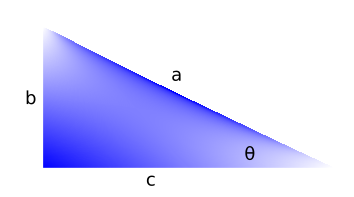
\includegraphics[scale=0.5]{imgsAux/triangulo.png}\\
\end{center}
Donde:
\[a=a, b=x \& c=\sqrt{a^{2}-x^{2}}\]
Partiendo de esto obtendremos:
\[\sin(\theta)= \frac{x}{a},\;\;\; x=a\sin(\theta),\;\;\; dx=a\cos(\theta)d\theta\]
Con ello sustituyendo a $x$ tendremos:
\[\sqrt{a^{2}-x^{2}}\Rightarrow \sqrt{a^{2}-a^{2}\sin^{2}(\theta)} \Leftrightarrow \sqrt{a^{2}[1-\sin^{2}(\theta)]} \Leftrightarrow \sqrt{a^{2}\cos^{2}(\theta)}\;\;\;\;\; \therefore \sqrt{a^{2}-x^{2}}=a\cos(\theta)\]
\subsubsection{Caso II:}
\begin{center}
  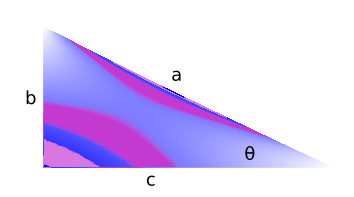
\includegraphics[scale=0.5]{imgsAux/triangulo1.png}\\
\end{center}
Donde:
\[a=\sqrt{a^{2}+x^{2}}, b=x \& c=a\]
Partiendo de esto obtendremos:
\[\tan(\theta)= \frac{x}{a},\;\;\; x=a\tan(\theta),\;\;\; dx=a\sec^{2}(\theta)d\theta\]
Con ello sustituyendo a $x$ tendremos:
\[\sqrt{a^{2}+x^{2}}\Rightarrow \sqrt{a^{2}+a^{2}\tan^{2}(\theta)} \Leftrightarrow \sqrt{a^{2}[1+\tan^{2}(\theta)]} \Leftrightarrow \sqrt{a^{2}\sec^{2}(\theta)}\;\;\;\;\; \therefore \sqrt{a^{2}+x^{2}}=a\sec(\theta)\]
\clearpage
\subsubsection{Caso III:}
\begin{center}
  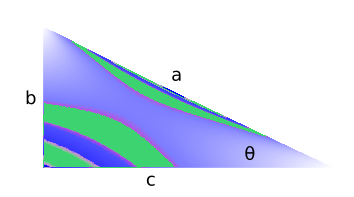
\includegraphics[scale=0.5]{imgsAux/triangulo2.png}\\
\end{center}
Donde:
\[a=x, b=\sqrt{x^{2}-a^{2}} \& c=a\]
Partiendo de esto obtendremos:
\[\sec(\theta)= \frac{x}{a},\;\;\; x=a\sec(\theta),\;\;\; dx=a\sec(\theta)\tan(\theta)d\theta\]
Con ello sustituyendo a $x$ tendremos:
\[\sqrt{x^{2}-a^{2}}\Rightarrow \sqrt{a^{2}\sec^{2}(\theta)-a^{2}} \Leftrightarrow \sqrt{a^{2}[\sec^{2}(\theta)-1]} \Leftrightarrow \sqrt{a^{2}\tan^{2}(\theta)}\;\;\;\;\; \therefore \sqrt{x^{2}-a^{2}}=a\tan(\theta)\]
\textit{\textbf{Aplicado ahora en alguna integral tendremos:}}\\
\[\int \frac{dx}{\sqrt{9+x^{2}}}\]
\textit{Solución}\\
De acuerdo con los casos que tenemos podemos aplicar el Caso II en el problema por lo que sustituyendo directamente tendremos $a=3$ \& $x=3\tan(\theta)$:
\[\int \frac{3\sec^{2}(\theta)}{3\sec(\theta)}d\theta \; \Leftrightarrow \; \int \sec(\theta)d\theta = \ln\left|\sec(\theta)+\tan(\theta)\right|+C\]
Finalmente sustituiremos los valores de las identidades trigonométricas con sus respectivos valores de triangulo:
\[\int \frac{dx}{\sqrt{9+x^{2}}}= \ln\left|\frac{\sqrt{9+x^{2}}}{3}+\frac{x}{3}\right|+C\]
\\\vspace{0.5cm}
\[\int\frac{dx}{\sqrt{x^{2}+2x+26}}\]
\textit{Solución}\\
Para abordar este problema a traves de sustitución trigonométrica es necesario reducir el polinomio interno de la raíz cuadrada, por lo primer rescribiremos la integral:
\[\int \frac{dx}{\sqrt{x^{2}+2x+25+1}}\Leftrightarrow \int \frac{dx}{\sqrt{(x+1)^{2}+5^{2}}}\]
Ahora una vez reduciendo esto haremos un cambio de variable el cual sera $u=x+1$ \& $du=dx$, reescribiendo la integral tenemos:
\[\int \frac{du}{\sqrt{u^{2}+5^{2}}}\]
Con esto podemos aplicar directamente el Caso II, por lo que saltando todo el cambio de variable hacia $\theta$ debido al anterior ejemplo tendremos:
\[\int \frac{du}{\sqrt{u^{2}+5^{2}}}=\ln\left|\sec(\theta)+\tan(\theta)\right|+C\]
Lo cual es:
\[\int \frac{du}{\sqrt{u^{2}+5^{2}}}=\ln\left|\frac{\sqrt{u^{2}+25}}{5}+\frac{u}{5}\right|+C\]
Sustituyendo el valor de $u$ por su respectivo valor en $x$:
\[\int\frac{dx}{\sqrt{x^{2}+2x+26}}=\ln\left|\frac{{\sqrt{(x+1)^2+25}}}{5}+\frac{x+1}{5}\right|+C\]
\\\vspace{0.5cm}
\textbf{Ejercicio propuesto:}
\begin{enumerate}
  \item \[\int\frac{\sqrt{x^{2}-4}}{x}dx\]
\end{enumerate}
\clearpage

\section{Ecuaciones Diferenciales}
\textbf{Definición:} Se dice que una Ecuación Diferencial (ED) que contiene las derivadas de una o más variables dependientes, con respecto a una o más variables independientes es conocida como una ED.\\
\textit{Nota:} Para referirse a ellas, se clasifican a las ED's por:
\begin{itemize}
  \item Tipo
  \item Orden
  \item Linealidad
\end{itemize}
\subsection{Clasificación por Tipo}
Si una ED contiene solo derivadas ordinarias de una o más variables independientes, se dice que es una ED Ordinaria (EDO)
\\\textbf{Ejemplos:}
\[\frac{dy}{dx}+5y=e^{x}\;\;\;\;\;\;\frac{d^{2}y}{dx^{2}}-\frac{dy}{dx}+6y=0 \;\;\;\;\;\;\frac{dx}{dt}+\frac{dy}{dt}=2x+y\]
Una ED con derivadas parciales de una o más variables dependientes con respecto de dos o más variables independientes se llaman ED Parcial (EDP)
\\\textbf{Ejemplos:}\\
\[\frac{\partial^{2}u}{\partial x^{2}}+\frac{\partial^{2}u}{\partial y^{2}}=0;\;\;\;\;\;\; u=u(x,y)\]
\[\frac{\partial^{2}u}{\partial x^{2}}=\frac{\partial^{2}u}{\partial t^{2}}-2\frac{\partial u}{\partial t};\;\;\;\;\;\; u=u(x,t)\]
\[\frac{\partial u}{\partial y}=\frac{\partial u}{\partial x}; \;\;\;\;\;\; u=u(y)\;\;\&\;\;u=u(x)\]
\textit{Nota:} En todo o la mayor parte del curso las derivadas ordinarias escribiremos con la notación de Leibniz:
\[\frac{dy}{dx},\;\;\frac{d^{2}y}{dx^{2}},\;\;\frac{d^{3}y}{dx^{3}},\;\;\ldots\;\;,\frac{d^{n}y}{dx^{n}} \Rightarrow y',\;\;y'',\;\;y''',\;\;y^{n}\]
Entonces las EDO de los ejemplos quedan como:
\[y'+5y=e^{x}\;\;\;\;\;\;y''-y'+6y=0\;\;\;\;\;\;x'+y'=2x+y\]
\clearpage
\subsection{Clasificación por Orden}
El orden de una ED ya sea Ordinaria o Parcial, se defide de acuerdo a la derivada de mayor orden\\
\textbf{Ejemplos:}
\[\frac{d^{2}y}{dx^{2}}+5\left(\frac{dy}{dx}\right)^{3}-4y=e^{x}\]
Encontrado los datos tendremos:
\begin{itemize}
  \item $\frac{d^{2}y}{dx^{2}}$ Es una componente diferencial de Orden 2
  \item $5\left(\frac{d^y}{dx}\right)^{3}$ Es una componente diferencial de Orden 1
\end{itemize}
$\therefore$ Esta ED es de Orden 2\\
\textit{Nota:} En ocasiones las EDO's de $1^{er}$ Orden se escriben como:
\[y'=f(x,y) \;\;\;\Rightarrow\;\;\; M(x,y)dx+N(x,y)dy=0;\]
\[N(x,y)dy=-M(x,y)dx;\;\;\;N(x,y)\frac{dy}{dx}=-M(x,y)\]
\[\frac{dy}{dx}=-\frac{M(x,y)}{N(x,y)}\]

\subsection{Clasificación por Linealidad}
Una EDO de Orden n-esimo es lineal, si $F(x,y,y',y'',y''',\ldots,y^{n})=0$ es lineal o $y,y',y'',y''' ,\ldots,y^{n}$, es decir, una EDO de Orden n es lineal si la podemos escribir como:
\[a_{n}(x)\frac{d^{n}y}{dx^{n}}+\left( a_{n-1}(x)\frac{d^{n-1}y}{dx^{n-1}}+\ldots+a_{2}(x)\frac{d^{2}y}{dx^{2}}+a_{1}(x)\frac{dy}{dx}+a_{0}y\right)=g(x)\ldots\ldots\ldots\ldots(*)\]
Si vemos la definición de $(*)$ sabemos que es una combinación lineal.\\
En la combinación lineal observamos que las propiedades y caracteristicas de una EDO lineal son como:
\begin{enumerate}
  \item La variable dependiente $(y)$ y todas sus derivadas $y',y'',y''',\ldots,y^{n}$ son de $1^{er}$ grado, es decir, la potencia de cada término en que interviene la variable $y$ es 1
  \item Los coeficientes $\left(a_{0},a_{1},a_{2},\ldots,a_{n}\;\;de\;\;y,y',y'',\ldots,y^{n}\right)$ dependen unicamento de la variable $x$
\end{enumerate}
\textit{Nota:}Una EDO no-lineal es simplemente una que no esta representada en combinación lineal, como:\\
\textbf{Ejemplo}
\[(1-y)y'+2y=e^{x}\;\;\;\;\;\;\frac{d^{2}y}{dx^{2}}+\sin(y)=0\;\;\;\;\;\;\frac{d^{4}y}{dx^{4}}+y^{2}=0\]
\clearpage
\section{Soluciones}
\subsection{Solución de una ED}
Uno de los objetivos primordiales del curso es resolver o encontrar soluciones de EDO's.\\
\textbf{Definición:} Cualquier función $\phi(x)$, definida en un intervalo $I$ y con al menos n-derivadas continuas en dicho intervalo de $I$, que al sustituirse en una EDO de n-esimo orden reduce a la ED en una identidad, se considera solución de dicha EDO.
\\\textbf{Ejemplos:}
\[a)\;\frac{dy}{dx}=xy^{\frac{1}{2}}\;\;;\;\;y=\frac{x^{4}}{16}\;\;\;\;|\;\;\;\;b)\;y''-2y'+y=0\;\;;\;\;y=xe^{x}\]
\textit{Solución} $a,b$, la cual derivaremos y sustituiremos los valores en las ecuaciones correspodientes, se procedera directamente:
\[\frac{x^{3}}{4}=x\left(\frac{x^{2}}{4}\right)\;\;\;\;\;\;\;\;\;\;\;\;\;\;\;\;\;\;\;\;\;\;\;\;\;|\;\;\;\;\;\;(x+2)e^{x}-2[(x+1)e^{x}]+xe^{x}=0\]
Finalmente resolviendo estas ecuaciones algebraicas podemos probar que la ED es correcta en primer instancia.\\
\textit{Nota:} Una solución de una ED que es identicamente a cero en un intervalo $I$ se llama solución trivial (Si $y\equiv0$)

\subsection{Solución explicita e implicita}
\textbf{Definición solución explicita:} Se dice que una solución es explicita, si en dicha solución la variable dependiente se expresa únicamente en términos de la variable independiente y constantes
\\\textbf{Ejemplos:}
\[y(x)=\frac{x^{2}}{2}+4\;\;\;\;\;\;\;\;\;\;\;\;y(x)=9x^{2}+5x+e^{5x}\]

\textbf{Definición solución implicita} Una relación $G(x,y)=0$ es una solución implicita de una EDO en un intervalo $I$, siempre que exista al menos una función $\phi(x)$ que satisfaga tanto a la relación como  a la ED en $I$
\\\textbf{Ejemplo:}
La relación $x^{2}+y^{2}=25$ es una solución implicita de la ED
\[\frac{dy}{dx}=-\frac{x}{y}\;\;\;\;\;\;\;en\;\;\;I=(-5,5)\]
\textit{Solución}\\
Derivamos implicitamente a la relación:
\[2x+2yy'=0 \;\Rightarrow\; 2yy'=-2x \;\Rightarrow\; y'=-\frac{2x}{2y}\;\Rightarrow\; y'=-\frac{x}{y}\]
Por otra parte:
\[\left|y\right|=\sqrt{25-x^{2}}\;\Rightarrow\;\phi_{1}(x)=\sqrt{25-x^{2}}\;\;\;\&\;\;\;\phi_{2}(x)=-\sqrt{25-x^{2}}\]
\clearpage
\subsection{Solución general, condiciones inciales\\Solución particular y unicidad de la solución}
Para que sea más ilustrativo este tema se mostrara el como se realiza a traves de una ecuación.\\
Sea $\frac{dy}{dx}=2x$, encontrar su solución general y su solución particular si $y(x=0)=1$
\\\textit{Solución}
\[\frac{dy}{dx}=2x\:\:\;\Rightarrow dy=2xdx\:\:\;\Rightarrow \int dy=\int 2xdx\]
En su solución general es decir que se tiene una familia de curvas bajo la constante $C$ de la integral obtendremos:
\[y(x)=x^{2}+C\;\;\;|\;C \in \mathbb{R}\;\;\;\;(Sol.\;\;general)\]
Para su solución particular usaremos la condición inicial dada al inicio, obteniendo lo siguiente con $x=0$:
\[y(0)\equiv 1 \;\;\;\;\;\;\;\;1=(0)^{2}+C \Rightarrow C=1\;\;\;\;\;\;\;\;\therefore y(x)=x^{2}+1\;\;\;\;(Sol.\;\;particular)\]
\section{Método de separación de variables para EDO-$1^{er}$ Orden}
Sea $\frac{dy}{dx}=f(x,y)$, donde sabemos o definimos que $f(x,y)=\frac{h(x)}{g(y)}$\\
Solucionando esto tendremos que de acuerdo a la ED $\frac{dy}{dx}=\frac{h(x)}{g(y)}$, reacomodando los terminos y tomando en cuenta que los terminos del diferencial $dx$ y $dy$ respectivamente tendremos que "multiplicar" por un diferencial en ambas partes de la ED, este diferencial es $dx$.\\
Obteniendo:
\[dy=\frac{h(x)}{g(y)}dx\]
Reacomodando las funciones de $f(x,y)$:
\[g(y)dy=h(x)dx\]
Finalmente integrando:
\[\int g(y)dx=\int h(x)dx\]
Obtendremos:
\[G(y)=H(x)+C \Leftrightarrow G(y)-H(x)=C\]
\textbf{Ejemplo}\\
Integrar las siguiente ED's:
\[a)\;\;\;\;\;\;\frac{dy}{dx}=\frac{2xy}{(x^{2}-1)(y^{3}+3)}\]
\textit{Solución}
\[dy=\frac{2xy}{(x^{2}-1)(y^{3}+3)}dx\]
\[\frac{(y^{3}+3)}{y}dy=\frac{2x}{x^{2}-1}dx \ldots\ldots(0)\]
Procederemos a resolver $(0)$ separando las integrales necesarias si es necesario y con las tecnicas previamente aprendidas:
\[\int\frac{y^{3}}{y}dy+3\int\frac{dy}{y}=\int\frac{2x}{x^{2}-1}dx\]
Resolviendo:
\[\frac{y^{3}}{3}+3\ln\left|y\right|=\ln\left|x^{2}-1\right|+C\]
\clearpage
\[b)\;\;\;\;\;\;y'=xy+x-2y-2;\;\;\;y(0)=2\]
\textit{Solución}
\[\frac{dy}{dx}=xy+x-2y-2 \;\Rightarrow\;\frac{dy}{dx}=x(y+1)-2(y+1)\]
\[\Rightarrow\frac{dy}{dx}=(x-2)(y+1)\;\Rightarrow\;\frac{dy}{y+1}=(x-2)dx\]
\[\int\frac{dy}{y+1}=\int(x-2)dx\]
Solucionando la integral:
\[\ln\left|y+1\right|=\frac{x^{2}}{2}-2x+C\]
Ahora para resolver el apartado de las condiciones iniciales para encontrar una solución particular procederemos inicialmente a reducir o expandira la ecuación, con:
\[e^{\ln|y+1|}=e^{x^{2}-2x+C} \Leftrightarrow y+1=e^{x^{2}-2x+C}\]
De modo que la constante C que interviene en el valor exponencial del lado de $x$ la podemos separar e inmediatamente decir que es:
\[y+1=Ce^{x^{2}-2x}\Rightarrow y=Ce^{x^{2}-2x}-1\]
De modo que ya tendremos una función $y(x)$, ahora aplicando las condiciones tendremos:
\[2=Ce^{x^{2}-2x}-1\;\Rightarrow 2=Ce^{0}-1\;\Rightarrow 2=C-1\;\Rightarrow C=3\]
\[\therefore y(x)=3e^{x^{2}-2x}-1\]
\\\vspace{0.5cm}
\[c)\;\;\frac{dy}{dx}(x^{2}+1)\tan(y)=x\]
\textit{Solución}
\[\tan(y)\frac{dy}{dx}=\frac{x}{x^{2}+1}\;\;\;\;\;\;\Rightarrow\;\;\;\;\;\; \tan(y)dy=\frac{x}{x^{2}+1}dx\]
\[\int \tan(y)dy=\int\frac{x}{x^{2}+1}dx\]
Hint: $\tan(y)=\frac{\sin(y)}{\cos(y)}$ por cambio de variable en dicha integral
\[\int\frac{\sin(y)}{\cos(y)}dy=\int\frac{x}{x^{2}+1}dx\]
\[-\ln\left|\cos(y)\right|=\frac{1}{2}\ln\left|x^{2}+1\right|+C\]
\clearpage
\textbf{Ejercicios propuestos:}
\begin{enumerate}
  \item \[y'=\frac{(x-2)(y-1)(y+3)}{(x-1)(x+3)(y-2)}\]
  \item \[y'=\frac{\sin(x)+e^{2y}\sin(x)}{3e^{y}+e^{y}\cos(2x)}\]
  \item \[y'=\frac{y+1}{\sqrt{x}+\sqrt{xy}}\]
  \item \[\left(y\ln(x)\right)^{-1}y'=\left(\frac{x}{y+1}\right)^{2}\]
  \item \[y'=\frac{xy+3y+x-3}{xy+2y-x-2}\]
\end{enumerate}

\section{Ecuaciones Homógeneas}
Una función $f(x,y)$ es homógenea de grado $n$, si en sus argumentos si cumple lo siguiente:\\
\[f(tx,ty)=t^{n}f(x,y)\]
\textbf{Ejemplo:}
\\Sea $f(x,y)=x^{2}+y^{2}-2xy$, verificar que es una función de grado $2$:\\
\textit{Solución}
\[f(tx,ty)=t^{2}x^{2}+t^{2}y^{2}-2txty\;\;\;=\;\;\;t^{2}x^{2}+t^{2}y^{2}-2t^{2}xy\]
\[=t^{2}(x^{2}+y^{2}-2xy)\;\;\;\Rightarrow\;\;\;t^{2}f(x,y)\]
Para n=0, se tiene una función de grado $0$\\
\textbf{Ejemplo:}\\
Sea $f(x,y)=\frac{x^{2}-y^{2}}{x^{2}+y^{2}}$
\textit{Solución}
\[f(tx,ty)=\frac{t^{2}x^{2}-t^{2}y^{2}}{t^{2}x^{2}+t^{2}y^{2}}\;\;\;\Leftrightarrow\;\;\;f(tx,ty)=\frac{t^{2}}{t^{2}}\frac{x^{2}-y^{2}}{x^{2}+y^{2}}\;\;\;\therefore t^{0}\]
\clearpage
\subsection{Ecuaciones Homógeneas en ED}
Para resolver ED es necesario plantear un modelo de cambio de variable, el cual te permitira resolver la ecuación diferencial de grado $n$\\
Resolver las siguientes ED's homógeneas:
\[xy'=\sqrt{x^{2}-y^{2}}+y\]
\textit{Solución}
\[y'=\frac{\sqrt{x^{2}-y^{2}}+y}{x}\]
\[y'=\sqrt{\frac{x^{2}}{x^{2}}-\frac{y^{2}}{x^{2}}}+\frac{y}{x}\;\;\;\;\;\ldots\;\;\;\;y'=\sqrt{1-\frac{y^{2}}{x^{2}}}+\frac{y}{x}\rightarrow (1)\]
\[f(x,y)=\sqrt{1-\frac{y^{2}}{x^{2}}}+\frac{y}{x}\]
\[f(tx,ty)=\sqrt{1-\left(\frac{ty}{tx}\right)^{2}}+\frac{ty}{tx}\;\;\;\;\;\;\;\;\therefore\;\;Es\;\;Hom\acute{o}genea\]
Por lo tanto propondremos el siguiente cambio de variable:
\[u=\frac{y}{x}\;\;\;\;\;\;\;\;\;\;\;\;y=ux\;\;\;\;\Rightarrow\;\;\;\;y'=u+x\frac{du}{dx}\rightarrow(2)\]
Ahora sustituimos $(2)$ en $(1)$:
\[u+xu'=\sqrt{1-u^{2}}+u\]
\[xu'=\sqrt{1-u^{2}}\;\;\;\;\Leftrightarrow\;\;\;\;x\frac{du}{dx}=\sqrt{1-u^{2}}\]
Ahora solo procederemos a resolver la ED, no olvidando el cambio de variable:
\[xdu=\sqrt{1-u^{2}}dx\;\;\;\;\Leftrightarrow\;\;\;\;\frac{du}{\sqrt{1-u^{2}}}=\frac{dx}{x}\]
\[\int\frac{du}{\sqrt{1-u^{2}}}=\int\frac{dx}{x}\]
Resolviendo la integral tendremos:
\[\arcsin(u)=\ln(x)+C\;\;\;\;\Leftrightarrow\;\;\;\;u=\sin\left(\ln\left|x\right|+C\right)\]
Sustituyendo el valor de $u$
\[\frac{y}{x}=\sin\left(\ln\left|x\right|+C\right)\;\;\;\;\Leftrightarrow\;\;\;\;y=x\sin\left(\ln\left|x\right|+C\right)\]

\clearpage
\[(x-y)dx+(x+y)dy=0\]
\textit{Solución}
\[(x-y)dx+(x+y)dy=0\;\;\;\;\Leftrightarrow\;\;\;\;(x+y)dy=(y-x)dx\]
\[\frac{dy}{dx}=\frac{(y-x)}{(x+y)}\rightarrow(1)\;\;\;\;\Rightarrow\;\;\;\;f(x,y)=\frac{(y-x)}{(x+y)}\]
Entonces comprobaremos si $f(x,y)$ es homógenea:
\[f(tx,ty)=\frac{ty-tx}{tx+ty}\;\;\;\;=\;\;\;\;\frac{t}{t}\frac{y-x}{x+y}\;\;\;\;\therefore\;Es\;\;hom\acute{o}genea\]
\[f(x,y)=\frac{x}{x}\frac{\cfrac{y}{x}-1}{1+\cfrac{y}{x}}\;\;\;\;=\;\;\;\;\frac{\cfrac{y}{x}-1}{1+\cfrac{y}{x}}\]
Entonces con el cambio de variable propondremos:
\[u=\frac{y}{x}\;\;\;\;\;\;\;\;\;\;\;\;y=ux\;\;\;\;\;\;\;\;\;\;\;\;y'=u+x\frac{du}{dx}\rightarrow(2)\]
Ahora sustituyendo $(2)$ en $(1)$:
\[u+x\frac{du}{dx}=\frac{u-1}{u+1}\;\;\;\;\Leftrightarrow \;\;\;\;x\frac{du}{dx}=\frac{u-1}{u+1}-u\]
\[x\frac{du}{dx}=\frac{u-1-u(u+1)}{u+1}\;\;\;\;\Leftrightarrow \;\;\;\;x\frac{du}{dx}=\frac{u-1-u^{2}-u}{u+1}\]
\[x\frac{du}{dx}=-\frac{1+u^{2}}{u+1}\;\;\;\;\Leftrightarrow \;\;\;\;\frac{u+1}{u^{2}+1}du=-\frac{dx}{x}\]
\[\int\frac{u+1}{u^{2}+1}du=-\int\frac{dx}{x}\]
\[\int\frac{u}{u^{2}+1}du+\int\frac{du}{u^{2}+1}=-\int\frac{dx}{x}\]
Resolviendo cada integral tendremos los siguientes resultados:
\[\frac{1}{2}\ln\left|u^{2}+1\right|+\arctan(u)=-\ln\left|x\right|+C\]
\[\frac{1}{2}\ln\left|u^{2}+1\right|+\arctan(u)+\ln\left|x\right|=C\]
Aplicando leyes de los logaritmos:
\[\ln\left|x\left(u^{2}+1\right)^{\frac{1}{2}}\right|+\arctan(u)=C\]
Sustituyendo los valores de $u$
\[\ln\left|x\left(\left(\frac{y}{x}\right)^{2}+1\right)^{\frac{1}{2}}\right|+\arctan\left(\frac{y}{x}\right)=C\]

\clearpage
\[ydx+x\left(\ln(x)-\ln(y)-1\right)dy=0;\;\;\;\;y(1)=e\]
\textit{Solución}
\[ydx+x(\ln(x)-\ln(y)-1)dy=0\;\;\;\;\Leftrightarrow\;\;\;\;ydx+x\left\{\ln(x)-\right[\ln(y)+\ln(e)\left]\right\}dy=0\]
\[ydx+x\left[\ln(x)-\ln(ey)\right]dy=0\;\;\;\;\Leftrightarrow\;\;\;\;ydx+x\ln\left(\frac{x}{ey}\right)dy=0\]
\[x\ln\left(\frac{x}{ey}\right)dy=-ydx\;\;\;\;\Leftrightarrow\;\;\;\;x\ln\left(\frac{x}{ey}\right)\frac{dy}{dx}=-y\]
\[\frac{dy}{dx}=-\frac{y}{x\ln\left(\frac{x}{ey}\right)}\;\;\;\;\Leftrightarrow\;\;\;\;\frac{dy}{dx}=\frac{y}{x\ln\left(\frac{ey}{x}\right)}\]
Reescribiremos lo siguiente:
\[f(x,y)=\frac{y}{x\ln\left(\frac{ey}{x}\right)}\]
\[f(tx,ty)=\frac{t}{t}\frac{y}{x\ln\left(\frac{t}{t}\frac{ey}{x}\right)}\;\;\;\;\therefore\;\;Es\;\;hom\acute{o}genea\]
Proponiendo el cambio de variable:
\[u=\frac{y}{x};\;\;\;\;y=ux;\;\;\;\;\frac{dy}{dx}=u+x\frac{du}{dx}\]
Entonces:
\[u+x\frac{du}{dx}=\frac{u}{\ln(eu)}\;\;\;\;\Leftrightarrow\;\;\;\;x\frac{du}{dx}=\frac{u-u\ln(eu)}{\ln(eu)}\]
\[du=\frac{1}{x}\frac{u-u\ln(eu)}{\ln(eu)}dx\;\;\;\;\Leftrightarrow\;\;\;\;\frac{\ln(eu)}{u-u\ln(eu)}du=\frac{dx}{x}\]
Resolviendo la integral:
\[\int\frac{\ln(eu)}{u-u\ln(eu)}du=\int\frac{dx}{x}\]
Para resolver, podemos proponer el cambio de variable, el cual quedaria con lo siguiente
\[v=u-u\ln(eu)\;\;\;\;\Rightarrow\;\;\;\;dv=1-\ln(eu)+1\;\;\;\therefore\;dv=-\ln(eu)\]
Ahora:
\[-\int\frac{dv}{v}=\int\frac{dx}{x}\;\;\;\;\Leftrightarrow\;\;\;\;-\ln|v|=\ln|x|+C\]
\[-\ln|u-u\ln(eu)|=\ln|x|+C\;\;\;\;\Leftrightarrow\;\;\;\;-\ln\left|\frac{y}{x}-\frac{y}{x}\ln\left(\frac{ey}{x}\right)\right|=\ln|x|+C\]
Solución general:
\[\ln\left|\frac{y}{x}-\frac{y}{x}\ln\left(\frac{ey}{x}\right)\right|+\ln|x|+C=0\]
Solución particular $y(1)=e$:
\[\ln\left|e-e\ln(e)^{2}\right|+C=0\;\;\;\;\Leftrightarrow\;\;\;\;\ln\left|e-2e\ln(e)\right|+C=0\]
Donde $\ln|e|=\ln|-e|=1$
\[\ln|e-2e|+C=0\;\;\;\;\Leftrightarrow\;\;\;\;\ln|-e|+C=0\;\;\;\therefore\;\;C=-1\]
Solución:
\[\ln\left|\frac{y}{x}-\frac{y}{x}\ln\left(\frac{ey}{x}\right)\right|+\ln|x|-1=0\]
\clearpage

\section{Ecuaciones Exactas}
Sea $z=f(x,y)$ una función de dos variables con primeras derivadas parciales continuas en una región $R\tiny{xy}$ del plano $xy$, entonces su diferencial es:
\[dz=\frac{\partial{f(x,y)}}{\partial{x}}dx+\frac{\partial{f(x,y)}}{\partial{y}}dy\;\;\;\;(i)\]
Si $f(x,y)=C;\;\;\;C=cte$, entonces $(i)$ se transforma en:
\[\frac{\partial{f(x,y)}}{\partial{x}}dx+\frac{\partial{f(x,y)}}{\partial{y}}dy=0\;\;\;\;(ii)\]
Dada una familia de funciones $f(x,y)=C$ puede generar una ED de primer orden calculando la diferencial en ambos lados de la igualdad:
\\
\textbf{Ejemplo:}
\\
Si $x^{2}-5xy+y^{2}=C$ el inciso $(ii)$ provee la ED de primer orden
\[(2x-5y)dx+(-5x+2y)dy=0\]
De tal forma que la ED es de la forma:
\[M(x,y)dx+N(x,y)dy=0\;\;\;\;(iii)\]
Se llama ED exacta si su primer miembro es la diferencial total de una función $f(x.y)$, es decir:
\[M(x,y)dx+N(x,y)dy=df(x,y)=\frac{\partial{f(x,y)}}{\partial{x}}dx+\frac{\partial{f(x,y)}}{\partial{y}}dy\]
Entonces obtener la solución de una ED exacta consiste en encontrar una función $f(x,y)=C$, tal que su diferencial sea exactamente la ED que se pretende resolver.
\\
\textbf{Ejemplo:}
\\
Supongase que se tiene la ED:
\[2xydx+x^{2}dy=9\]
Que es exacta ya que proviene de la función:
\[z=f(x,y)=x^{2}y\]
Donde podemos observar que:
\[\frac{\partial{f}}{\partial{x}}=2xy;\;\;\;\frac{\partial{f}}{\partial{y}}=x^{2}\]
\[\Rightarrow\;\frac{\partial{f}}{\partial{x}}dx+\frac{\partial{f}}{\partial{y}}dy=2xydx+x^{2}dy=0\]
\[\Rightarrow\;\;M(x,y)=\frac{\partial{f}}{\partial{x}}\;\;\;(iv)\]
\[\Rightarrow\;\;N(x,y)=\frac{\partial{f}}{\partial{y}}\;\;\;(v)\]
Ahora, si derivamos a la ecuaciones $(iv)$ y $(v)$, pero ahora con respecto a la otra variable respectivamente:
\[\frac{\partial{M}}{\partial{y}}=\frac{\partial}{\partial{y}}\frac{\partial{M}}{\partial{x}}=\frac{\partial^{2}{M}}{\partial{y}\partial{x}}\;\;\;\;(vi)\]
\[\frac{\partial{N}}{\partial{x}}=\frac{\partial}{\partial{x}}\frac{\partial{M}}{\partial{y}}=\frac{\partial^{2}{N}}{\partial{x}\partial{y}}\;\;\;\;(vii)\]
Continuando, como supusimos desde un inicio que las derivadas parciales de $f(x,y)$ son continuas, tendremos:
\[\frac{\partial{M}}{\partial{y}}\equiv \frac{\partial{N}}{\partial{x}}\;\;(viii)\;\;Condici\acute{o}n\;para\;que\;una\;ED\;sea\;exacta\]
\textit{Nota:} Por tanto la ED es exacta si se cumple la condicion $(viii)$\\
Para poder resolver una ED exacta recurriremos a las ecuaciones $(iv)$ o $(v)$, es decir, nos apoyaremos de dichas expresiones:
\[M(x,y)=\frac{\partial{f}}{\partial{x}}\;\;\;\;(ix)\]
\[N(x,y)=\frac{\partial{f}}{\partial{y}}\;\;\;\;(x)\]
Entonces si tomamos la ecuación $(ix)$ e integramos parcialmente respecto a $x$ obtenemos $f(x,y)$, de tal forma que:
\[f(x,y)=\int M(x,y)dx+h(y)\;\;\;\;(xi)\]
que es la solución buscada, solo falta hallar o determinar $h(y)$ que es una expresion que representa a la constante arbitraría de la integral anterior.
\\
Para determinar $h(y)$ se deriva a la $(xi)$ respecto de $y$ y se obtiene:
\[\frac{\partial{f}}{\partial{y}}=N(x,y)=\frac{\partial}{\partial{y}}\int M(x,y)dx + h'(y)\;\;\;(xii)\]
Que al despejar se tiene:
\[h'(y)=N(x,y)=-\frac{\partial}{\partial{y}}\int M(x,y)dx\;\;\;\;(xiii)\]
Y finalmente para conocer $h(y)$ se integra a $(xiii)$.
\\
\textit{Nota: }Resaltemos que para el caso de integrar con respecto a $y$ es el mismo procedimiento, solo cambia la variable con la que se trabaja\\
\clearpage
\textbf{Ejemplo:}
\\
\[2y\sin(x)\cos(x)dx+\sin^{2}(x)dy=0\]
\textit{Solución}\\
Paso 1: Determinar si la ecuación es exacta:
\[M(x,y)=2y\sin(x)\cos(x);\;\;\;\;N(x,y)=\sin^{2}(x)\]
\[\Rightarrow \frac{\partial{M}}{\partial{y}}=2\sin(x)\cos(x)\;\;\;\&\;\;\;\frac{\partial{N}}{\partial{x}}=2\sin(x)\cos(x)\]
\[\therefore\;\;\frac{\partial{M}}{\partial{y}}=\frac{\partial{N}}{\partial{x}}\;\;La\;ED\;es\;exacta\]
Paso 2: seleccionar que vamos a integrar (en este caso sobre x)
\[\frac{\partial{f}}{\partial{x}}=M(x,y)\]
\[\int\frac{\partial{f}}{\partial{x}}=\int M(x,y)\;\;\;\;\Leftrightarrow\;\;\;\;f(x,y)=2y\int\sin(x)\cos(x)dx\]
Paso 3: Resoviendo la integral:
\[f(x,y)=y\sin^{2}(x)+h(y)\;\;Soluci\acute{o}n\;general\]
Paso 4: Ahora derivando con respecto a $y$
\[\frac{\partial{f}}{\partial{y}}=\sin^{2}(x)+h'(y)\equiv N(x,y)=\sin^{2}(x)\]
\[\Rightarrow\;\;h'(y)=0\;\;\;\;\int h'(y)=\int 0\]
\[\therefore\;\;h(y)=C\]
\[f(x,y)=y\sin^{2}(x)+C\;\;Soluci\acute{o}n\;general\]
Ahora pensando en que $y(x)$
\[y(x)=\frac{C}{\sin^{2}(x)}\]
\clearpage
Algunos otros ejemplos son:
\[(ye^{xy}+2x-1)dx+(xe^{xy}-2y+1)dy=0\]
\textit{Solución}
\[M(x,y)=ye^{xy}+2x-1\;\;\;\&\;\;\;N(x,y)=xe^{xy}-2y+1\]
\[\frac{\partial{M}}{\partial{y}}=xye^{xy}+e^{xy}\;\;\;\&\;\;\;\frac{\partial{N}}{\partial{x}}=xye^{xy}+e^{xy}\]
\[\therefore\;\;\frac{\partial{M}}{\partial{y}}\equiv\frac{\partial{N}}{\partial{x}}\]
\[\int\frac{\partial{f}}{\partial{x}}dx=\int M(x,y)dx\]
\[f(x,y)=e^{xy}+x^{2}-x+h(y)\]
Ahora para encontrar $h(y)$
\[\frac{\partial{f}}{\partial{y}}=xe^{xy}+h'(y)\equiv N(x,y)=xe^{xy}-2y+1\]
\[h'(y)=1-2y\;\;\;\Rightarrow\;\;\;\int h'(y)dy=\int(1-2y)dy\]
\[h(y)=y-y^{2}+C\]
\[f(x,y)=e^{xy}+x^{2}-x-y^{2}+y+C\]
\[f(x,y)=e^{xy}+x^{2}-x-y^{2}+y=C\]
\vspace{0.5cm}\\
\[(2x+6y)dx+(2y-6x)dy=0\]
\textit{Solución}
\[M(x,y)=2x+6y\;\;\;\&\;\;\;N(x,y)=2y-6x\]
\[\frac{\partial{M}}{\partial{y}}=6\;\;\;\&\;\;\;\frac{\partial{N}}{\partial{x}}=-6\]
\[\therefore\;\;\frac{\partial{M}}{\partial{y}}\neq\frac{\partial{N}}{\partial{x}}\]
En el siguiente tema se mostrara el como se resulven ED de primer orden que no cumplen con la propiedad de ser una ED exacta.
\vspace{1.5cm}\\
\textbf{Ejercicios propuestos:}
\begin{enumerate}
  \item \[(3y^{2}+2y\sin(2x))=\left(\cos(2x)-6xy-4\frac{4}{1+y^{2}}\right)y'\]
  \item \[\left(y\sin(x)+\sin(y)+\frac{1}{x}\right)dx+\left(x\cos(y)-\cos(x)+\frac{1}{y}\right)dy=0\]
\end{enumerate}
\clearpage
\section{Factor Integrante $\mu(x,y)$}
En asos excepcinales, cuando $df(x,y)=M(x,y)dx+N(x,y)dy$ no representa una ED exacta, se conseguira hallando una función $\mu(x,y)$ tal que el $2^{do}$ miembro de la expresión anterior multipicado por $\mu(x,y)$, resulta en una diferencial total (exacta).
\[df(x,y)=\mu(x,y)M(x,y)dx+\mu(x,y)N(x,y)dy\]
¿Cómo hallar a $\mu(x,y)$?\\
Partimos del hecho de que la ED tiene que ser exacta
\[\frac{\partial}{\partial{y}}(\mu M)\equiv \frac{\partial}{\partial{x}}(\mu N)\;\;\;\Rightarrow\;\;\mu\frac{\partial{M}}{\partial{x}}+M\frac{\partial{\mu}}{\partial{x}}=\mu\frac{\partial{N}}{\partial{y}}+N\frac{\partial{\mu}}{\partial{y}}\]
\[\mu\left(\frac{\partial{M}}{\partial{y}}-\frac{\partial{N}}{\partial{x}}\right)=N\frac{\partial{\mu}}{\partial{x}}-M\frac{\partial{\mu}}{\partial{y}}\]
Ahora pasaremos la función $\mu$ del otro lado de modo que:
\[\frac{\partial{M}}{\partial{y}}-\frac{\partial{N}}{\partial{x}}=N\frac{1}{\mu}\frac{\partial{\mu}}{\partial{x}}-M\frac{1}{\mu}\frac{\partial{\mu}}{\partial{y}}\]
Donde sabemos que:
\[\frac{1}{\mu}\frac{\partial{\mu}}{\partial{y}}=\frac{\partial}{\partial{y}}\ln(\mu)\;\;\;\;\&\;\;\;\;\frac{1}{\mu}\frac{\partial{\mu}}{\partial{x}}=\frac{\partial}{\partial{x}}\ln(\mu)\]
Entonces:
\[\Rightarrow\;\;N\frac{\partial{\ln(\mu)}}{\partial{x}}-M\frac{\partial{\ln(\mu)}}{\partial{y}}=\frac{\partial{M}}{\partial{y}}-\frac{\partial{N}}{\partial{x}}\]
\vspace{0.5cm}
\[Caso\;\;(i)\;\;si\;\;\mu=\mu(x)\;\Rightarrow\;\frac{\partial{\ln(\mu)}}{\partial{y}}=0\]\\
\[\Rightarrow\;\;N\frac{d\ln(\mu)}{dx}=\frac{\partial{M}}{\partial{y}}-\frac{\partial{N}}{\partial{x}}\;\;\;\;\Rightarrow\;\;\;\;\frac{d\ln(\mu)}{dx}=\frac{\frac{\partial{M}}{\partial{y}}-\frac{\partial{N}}{\partial{x}}}{N}\]
\[\int d\ln(\mu)=\int\frac{\frac{\partial{M}}{\partial{y}}-\frac{\partial{N}}{\partial{x}}}{N}dx\]
\[\ln(\mu)=\int\frac{\frac{\partial{M}}{\partial{y}}-\frac{\partial{N}}{\partial{x}}}{N}dx\;\;\Leftrightarrow\;\;\mu(x)=e^{\int{\frac{\frac{\partial{M}}{\partial{y}}-\frac{\partial{N}}{\partial{x}}}{N}dx}}\]
\vspace{1cm}
\[Caso\;\;(i)\;\;si\;\;\mu=\mu(y)\;\Rightarrow\;\frac{\partial{\ln(\mu)}}{\partial{x}}=0\]\\
\[\Rightarrow\;\;-M\frac{d\ln(\mu)}{dy}=\frac{\partial{M}}{\partial{y}}-\frac{\partial{N}}{\partial{x}}\;\;\;\;\Rightarrow\;\;\;\;\frac{d\ln(\mu)}{dy}=\frac{\frac{\partial{N}}{\partial{x}}-\frac{\partial{M}}{\partial{y}}}{M}\]
\[\int d\ln(\mu)=\int\frac{\frac{\partial{N}}{\partial{x}}-\frac{\partial{M}}{\partial{y}}}{M}dy\]
\[\mu(y)=e^{\int\frac{\frac{\partial{N}}{\partial{x}}-\frac{\partial{M}}{\partial{y}}}{M}dy}\]
\clearpage
\textbf{Ejemplo:}
\[\left(3y^{2}\cot(x)+\sin(x)\cos(x)\right)dx-2ydy=0\]
\textit{Solución:}
\[\frac{\partial{M}}{\partial{y}}=6y\cot(x)\;\;\;\;\neq\;\;\;\;\frac{\partial{N}}{\partial{x}}=0\]
Propondremos $\mu=\mu(x)$:
\[\int\frac{\frac{\partial{M}}{\partial{y}}-\frac{\partial{N}}{\partial{x}}}{N}dx\;=\;\int\frac{6y\cot(x)}{-2y}dx\;=\;-3\int\cot(x)dx\]
\[=\;-3\ln|\sin(x)|\;\;=\;\;\ln\left|\sin(x)\right|^{-3}\]
Ahora:
\[\mu(x)=e^{\ln\left|\sin(x)\right|^{-3}}\;\;\Leftrightarrow\;\;\mu(x)=\sin^{-3}(x)=\csc^{3}(x)\]
Multiplicando por $\mu$ por la ED original:
\[\left(3y^{2}\csc^{3}(x)\cot(x)+\csc^{2}(x)\cos(x)\right)dx-2y\csc^{3}(x)dy=0\]
Resolviendo:
\[\frac{\partial{\bar{M}}}{\partial{y}}=6y\csc^{3}(x)\cot(x)\;\;\;\equiv\;\;\;\frac{\partial{\bar{N}}}{\partial{x}}=6y\csc^{3}(x)\cot(x)\]
\[\int\frac{\partial{f}}{\partial{y}}dy=-2\int y\csc^{3}(x)dy\]
Resolviendo:
\[f(x,y)=-y^{2}\csc^{3}(x)+h(x)\]
Derivando:
\[\frac{\partial{f}}{\partial{x}}=3y^{2}\csc^{3}(x)\cot(x)+h'(x)\equiv\bar{M}(x,y)=3y^{2}\csc^{3}(x)\cot(x)+\csc^{2}(x)\cos(x)\]
\[h'(x)=\csc^{2}(x)\cos(x)\;\;\Rightarrow\;\;\int h'(x)dx=\int\csc^{2}(x)\cos(x)dx\]
\[h(x)=\csc(x)+K\]
\[f(x,y)=-y^{2}\csc^{3}(x)+\csc(x)+K\]
\[K=-y^{2}\csc^{3}(x)+\csc(x)\]
\textbf{Ejercicios propuestos:}
\begin{enumerate}
  \item \(\displaystyle \left(x+y^{2}\right)dx-2xydy=0\)
  \item \(\displaystyle \left[2xy\ln\left(y\right)\right]dx+\left(x^{2}+y^{2}\sqrt{y^{2}+1}\right)dy=0\)
  \item \(\displaystyle \left[3x^{5}\tan\left(y\right)-2y^{3}\right]dx+\left[x^{6}\sec^{2}\left(y\right)+4x^{3}y^{4}+3xy^{2}\right]dy=0\)
\end{enumerate}
\clearpage
\section{Ecuaciones Lineales de $1^{er}$ Orden}
Dada la ED de la forma:
\[a_{1}\left(x\right)\frac{dy}{dx}+a_{2}\left(x\right)y=g\left(x\right)\;\;(i)\]
Si nomalizamos $(i)$ obtendremos:
\[\frac{dy}{dx}+\frac{a_{2}\left(x\right)}{a_{1}\left(x\right)}y=\frac{g\left(x\right)}{a_{1}\left(x\right)}\;\;(ii)\]
Y denotaremos lo siguiente:
\[\frac{a_{2}(x)}{a_{1}(x)}=p(x)\;\;\&\;\;\frac{g(x)}{a_{1}(x)}=q(x)\]
De tal forma que $(ii)$ lo reescribimos como:
\[\frac{dy}{dx}+p(x)y=q(x)\;\;\acute{o}\;\;y'+p(x)y=q(x)\;\;(ii)\]
A la ED $(ii)$ se le llama ED lineal-no homogénea.\\
El método de soluci para esta forma de la ED lineal-no homogénea de $1^{er}$ orden llamdado método de variación de la constante lo exponemos por medio del siguiente ejemplo:
\\
\textbf{Ejemplos:}
\\
Resolver:
\[y'+2xy=0\;\;(0)\]
\textit{Solución}\\
\[\frac{dy}{dx}=-2xy \Rightarrow \int\frac{dy}{y}=-2\int xdx \Rightarrow \ln\left|y\right|=-x^{2}+C\]
Sustituyendo el logaritmo:
\[y=e^{-x^{2}+C}\Rightarrow y=e^{C}e^{-x^{2}}\;\;\therefore y=Ce^{-x^{2}}\;\;(i)\]
La cual denotaremos a $(i)$ como la Solución homogénea.\\
Ahora proponemos sustituirlo en la siguiente ecuación, pero poniendo a $C$ en función de $x$, denotando:
\[y_{p}=C(x)e^{-x^{2}}\;\;(1)\]
Derivando incialmente:
\[\frac{dy}{dx}=C'(x)e^{-x^{2}}-2xC(x)e^{-x^{2}}\;\;(3)\]
Posteriormente escribimos la formula de la ED lineal-no homogénea, toamdo en consideración la forma de la ED al inicio $(0)$ con los valores de $(1)$ y $(2)$:
\[C'(x)e^{-x^{2}}-2xC(x)e^{-x^{2}}+2xCe^{-x^2}=2xe^{-x^{2}}\]
Resolviendo tendremos lo siguiente:
\[C'(x)e^{-x^{2}}=2xe^{-x^{2}}\Rightarrow C'(x)=2x \Rightarrow \int C'(x)dx=\int 2xdx\]
Resolviendo:
\[C(x)=x^{2}+C\]
Sustituyendo la Solución homogénea:
\[y(x)=\left(x^{2}+C\right)e^{-x^{2}}\Leftrightarrow y(x)=x^{2}e^{-x^{2}}+Ce^{-x^{2}}\]

\textbf{Ejercicios propuestos:}
\begin{enumerate}
  \item \(\displaystyle 2xy' -y=3x^{2}\)
  \item \(\displaystyle y'+\left(\cot(x)\right)y=2\csc(x)\;y\left(\frac{\pi}{2}\right)=1\)
\end{enumerate}
\section{Aplicaciones}
Una de las principales y comunes aplicaciones de las ED en ingeniería son en el uso y calculo de voltaje o corriente en los Circuitos RLC:
\begin{center}
  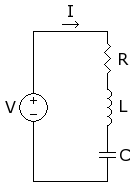
\includegraphics[scale=0.5]{imgsAux/rlc.png}
\end{center}
Dos principios físicos que rigen a los Circuitos RLC en serie son:
\begin{enumerate}
  \item La conservación de la Carga Electrica $(Q)$
  \item La conservación de la Energía
\end{enumerate}
Estas leyes de la conservación para Circuitos Electricos estan dados por la función formulada por G. Kirchhoff en 1859 y se llaman Leyes de Kirchhoff, las cuales no dicen:
\begin{enumerate}
  \item La corriente $I$ que circula a traves de cada uno de los elementos en serie debe ser la misma.
  \item La suma algebraica de los cambios instantáneos de potencial (Caídas de voltaje) alrededor de un Circuito cerrado debe ser cero y los voltajes de cada elemento son dados por:
  \begin{enumerate}
    \item Resistencia (R):
    \begin{itemize}
      \item Ley de Ohm
      \item \(\displaystyle V_{R}=IR \)
      \item \(\displaystyle V_{R}\) Caída de voltaje (Volts: V)
      \item \(\displaystyle I\) Intensidad de Corriente (Amperes: A)
      \item \(\displaystyle R\) Resistencia (Ohms: $\Omega$)
    \end{itemize}
    \item Inductor (Bobina) (L):
    \begin{itemize}
      \item Por las leyes de Faraday y la Ley de Lenz:
      \item \(\displaystyle V_{L}=L\frac{dI}{dt} \)
      \item \(\displaystyle V_{L}\) Voltaje (V)
      \item \(\displaystyle L\) Bobina o inductor (Henrys:hy)
      \item \(\displaystyle I\) Intensidad de Corriente (A)
    \end{itemize}
    \item Capacitor (C):
    \begin{itemize}
      \item \(\displaystyle V_{C}=\frac{Q}{C}\)
      \item \(\displaystyle V_{C}\) Voltaje (V)
      \item \(\displaystyle C\) Capacitor (Farads:Fd)
      \item \(\displaystyle Q\) Carga (Coulombs:C)
    \end{itemize}
  \end{enumerate}
\end{enumerate}
La fuerza electromotriz proporciona voltaje o energía potencial al Circuito. Si denotamos a $V$ como $E(t)$ y lo llamamos al voltaje  aplicado al tiempo $t$, entonces la Ley de Kirchhoff de conservación de la energía es:
\[E(t)=V_{R}+V_{L}+V_{C}\]
Sustituyendo esta formula con las definiciones de voltaje previamente explicadas, tendremos:
\[E(t)=IR+L\frac{dI}{dt}+\frac{1}{C}Q\]
Remarcando que \(\displaystyle I=\frac{dQ}{dt}\), entonces tendremos la ED:
\[E(t)=L\frac{d^{2}Q}{dt^{2}}+R\frac{dQ}{dt}+\frac{1}{C}Q\;\;ED\;de\;2^{do}\;orden\]
Para este caso de primer orden pensaremos en circuitos RL o RC, quedando ED de primer orden.
\subsection{RC}
Para este caso la ED sería:
\[R\frac{dQ}{dt}+\frac{1}{C}Q=E(t)\]
Normalizando:
\[\dot{Q}+\frac{1}{RC}Q=\frac{E(t)}{R}\]
\subsection{RL}
Para este caso la ED sería:
\[L\frac{dI}{dt}+RI=E(t)\]
Normalizando:
\[\dot{I}+\frac{R}{L}I=\frac{E(t)}{L}\]
\textit{Nota: Resolver como los ejercicios normales, solo cuidar las unidades con las que se trabajan}\\
\textbf{Ejercicios propuestos:}
\begin{enumerate}
  \item Considere un Circuito RC con $R=120\Omega$ y \(\displaystyle C=\frac{1}{1200}fd\) al tiempo $t=0$ se conecta una fuente de voltaje constante de $E(t)=120V$ si inicialmente la carga $Q=0$, determine como cambia la carga en el capacitor y la corriente del circuito.
  \item Se conecta un resistor $R=40\Omega$ y un Inductor $L=0.1hy$ con una fuente de $E(t)=110V$ si originalmente no hay corriente al $t=0$ $I(t=0)=0$ determine la corriente al tiempo $t$
\end{enumerate}
\section{Ecuaciones de Orden Superior}
La ED de orden superior cuenta con la siguiente forma:
\[a_{n}(x)\frac{d^{n}x}{dy^{n}}+a_{n-1}(x)\frac{d^{n-1}x}{dy^{n-1}}+\cdots+a_{2}\frac{d^{2}x}{dy^{2}}+a_{1}\frac{dx}{dy}+a_{0}(x)y=g(x)\]
Se dice llamar ED lineal de Orden-n donde los coeficientes $a_{i}(x)\;\forall i$ y $g(x)$ son funciones continuas en un intervalo I.\\
La ED se dice homogénea si $g(x)=0\;\forall x\in I$ de otra forma la ED es no-homogénea $g(x)\neq 0$
\\
\textbf{Ejemplo:}\\
\(\displaystyle 2y''+3y'-6y=0\;\;\;\;\;\;\;\;\;x^{3}y'''+6y'+10y=e^{x}\)\\
Donde podemos ver que la ED de la izquierda si es homogénea, mientras que la ED de la derecha es no-homogénea.\\
Supongamos que los coeficientos de la ED son números reales, entonces la ED se transforma en:
\[a_{n}y^{n}+a_{n-1}y^{n-1}+\cdots+a_{2}y''+a_{1}y'+a_{0}y=g(x)\]
A esta ecuación se le llama ED lineal de coeficientes constantes.\\
\textbf{Ejemplo:}\\
\(\displaystyle y'''+2y''+y'=e^{x}\;\;\;\;\;\;\;\;\;xy''+2y'+xy=0\)\\
\(\displaystyle y'''-y''=12x^{2}+6x\)\\
Donde podemos ver que las dos primeras ecuaciones de la izquierda son ED's con coeficientes constantes, mientras la ED de la derecho es una ED con coeficientes variables.
\clearpage
\subsection{Problemas de valor inicial}
Para una ED de orden-n sobre un intervalo I el problema de valor inicial consiste en que la ED y las n-condiciones, las cuales son:
\[y(x_{0})=y_{0},\;y'(x_{0})=y_{1},\;y''(x_{0})=y_{2},\;\cdots,\;y^{n-1}(x_{0})=y_{n-1}\]
Para cualquier punto $x_{0}\in I$ tendremos al Teorema de superposición:\\
\textbf{Teorema: (Teorema de superposición)}\\
Sean \(\displaystyle y_{1},\;y_{2},\;\cdots,\;y_{k}\) soluciones de la ED-homogénea de orden-n en un intervalor I.\\
Entonces \(\displaystyle C_{1}y_{1},\;C_{2}y_{2},\;\cdots,\;C_{k}y_{k}\) también son soluciones de la ED-homogénea, así como la combinación lineal de estas soluciones, es decir:
\[C_{1}y_{1}+C_{2}y_{2}+\cdots+C_{k}y_{k}=y(x)\] Que es la solución de la ED.\\
\textbf{Corolario:}
\begin{enumerate}
  \item Un múltiplo constante \(\displaystyle y=C_{i}y_{i}(x)\) de una solución \(\displaystyle y_{i}(x)\) es una ED lineal homogénea, es también solución
  \item Una ED lineal homogénea posee siempre la solución trivial \(\displaystyle y(x)=0\)
\end{enumerate}
\subsection{Ecuaciones lineales homogeneas de coeficientes constantes}
Sea dada la ED donde los coeficientes \(\displaystyle a_{i}\forall i\) son constantes reales:
\[a_{n}y^{n}+a_{n-1}y^{n-1}+\cdots+a_{2}y''+a_{1}y'+a_{0}y=0\]
Consideremos la ecuación asociada (o caracteristica) de la forma:
\[a_{n}\lambda^{n}+a_{n-1}\lambda^{n-1}+\cdots+a_{2}\lambda^{2}+a_{1}\lambda+a_{0}=0\]
Donde los \(\displaystyle \lambda\) son raíces o ceros de la ecuación asociada, entre las cuales pueden haber raíces multiples y/o complejas.\\
Por ello:
\begin{enumerate}
  \item Raíces Reales y distintas
  \begin{itemize}
    \item Si \(\displaystyle \lambda_{1},\;\lambda_{2},\;\cdots,\;\lambda_{n}\) son reales y distintas, la solución de la ED-lineal-homogénea es de la forma:
    \item \(\displaystyle y(x)=C_{1}e^{\lambda_{1}x}+C_{2}e^{\lambda_{2}x}+\cdots+C_{n}e^{\lambda_{n}x}\)
  \end{itemize}
  \item Raíces Reales multiples:
  \begin{itemize}
    \item Las raices de la ecuación asociada son reales, pero algunas son iguales, denotados por: \(\displaystyle \lambda_{1}=\lambda_{2}=\cdots=\lambda_{k}=\bar{\lambda}\); de modo que \(\displaystyle \bar{\lambda}\) es una raíz k-multiple de la solución, mientras que las demas (n-k) raíces son distintas, la solución es de la forma:
    \item \(\displaystyle y(x)=C_{1}e^{\bar{\lambda_{1}}x}+C_{2}xe^{\bar{\lambda_{2}}x}+\cdots+C_{k}x^{k-1}e^{\bar{\lambda_{n}}x}+C_{k+1}e^{\lambda_{k+1}x}+\cdots+C_{n}e^{\lambda_{n}x}\)
  \end{itemize}
  \item Raíces Complejas (Imaginarias) y distintas
  \begin{itemize}
    \item Si \(\displaystyle \lambda_{j}=\alpha_{j}\pm i\beta_{j}\) son distintos entre todas las soluciones, es decir  \(\displaystyle\lambda_{1}\neq\lambda_{2}\neq\cdots\neq\lambda_{k}\), las solución quedaria escrita como:
    \item \(\displaystyle y(x)=C_{1}e^{\alpha_{1}x}\cos\left(\beta_{1}x\right)+C_{2}e^{\alpha_{2}x}\sin\left(\beta_{2}x\right) + \cdots + C_{k}e^{\alpha_{k}x}\sin\left(\beta_{k}x\right)+C_{k+1}e^{\lambda_{k+1}x}+\cdots+C_{n}e^{\lambda_{n}x}\)
    \item \textit{Nota:} Recordemos que para este caso: \(\displaystyle e^{i\beta x}=\cos\left(\beta x\right)\) y \(\displaystyle e^{-i\beta x}=\sin\left(\beta x\right)\)
  \end{itemize}
  \item Raíces Complejas multiples:
  \begin{itemize}
    \item Al igual que las raíces reales multiples estas se acompañan por un valor un valor multiplicativo $x$ por cada raiz repetida.
  \end{itemize}
\end{enumerate}
\textit{Nota:} para resolver y encontrar raíces de cualquier tipo es necesario estudiar el tema de División sintetica.
\printindex
\end{document}
